\documentclass[tikz]{standalone}

\usetikzlibrary{calc}

\colorlet{FilledSurface}{blue!20}
\colorlet{FilledSurfaceGroupOne}{blue!20}
\colorlet{FilledSurfaceGroupTwo}{red!20}
\colorlet{FilledSurfaceGroupThree}{green!20}
\colorlet{FilledSurfaceGroupFour}{magenta!20}
\colorlet{FormulaBackground}{green!10}
\colorlet{FormulaFrame}{green}


\begin{document}
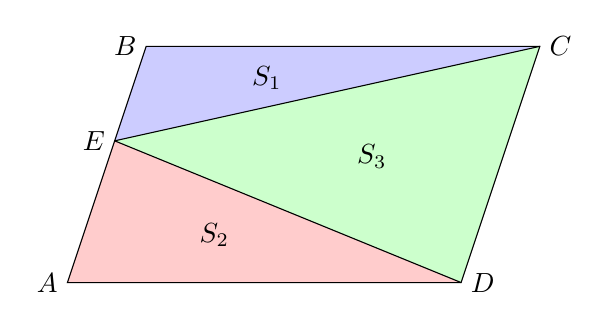
\begin{tikzpicture}

    \coordinate (A) at (0, 0);
    \coordinate (B) at (1, 3);
    \coordinate (C) at (6, 3);
    \coordinate (D) at (5, 0);

    % Punto arbitrario paralelos en lado AB
    \coordinate (E) at ($(A)!0.6!(B)$);

    \fill[FilledSurfaceGroupOne] (B) -- (C) -- (E);
    \fill[FilledSurfaceGroupTwo] (A) -- (D) -- (E);
    \fill[FilledSurfaceGroupThree] (C) -- (D) -- (E);

    \draw
    (A) node[left] {$A$}
    -- (B) node [left] {$B$}
    -- (C) node [right] {$C$}
    -- (D) node [right] {$D$}
    -- cycle;
    \draw (E) node [left] {$E$} -- (C);
    \draw (E) -- (D);

    \node at (barycentric cs:B=1,C=1,E=1) {$S_1$};
    \node at (barycentric cs:A=1,D=1,E=1) {$S_2$};
    \node at (barycentric cs:C=1,D=1,E=1) {$S_3$};
\end{tikzpicture}
\end{document}
